\documentclass[12pt]{article}
\usepackage{fancyhdr}
\usepackage{amsmath}
\usepackage{amsthm}
\usepackage{mathtools}
\usepackage{enumitem}
\usepackage[Export]{adjustbox}
\usepackage{cancel}
\usepackage{algorithm}
\usepackage[noend]{algpseudocode}
\usepackage{graphicx}
\usepackage[margin = 1in]{geometry}
\usepackage{blindtext}
\usepackage[section]{placeins}
\usepackage{xcolor,listings}
\usepackage{textcomp}
\usepackage[utf8]{inputenc}
\lstset{upquote=true}
\lstdefinestyle{myCustomRStyle}{
	language=R,
	backgroundcolor = \color{lightgray!10!white},
	numbers=left,
	stepnumber=1,
	numbersep=10pt,
	tabsize=2,
	showspaces=false,
	breaklines=true
	showstringspaces=false,
	basicstyle=\footnotesize\ttfamily,
	keywordstyle=\bfseries\color{blue!50!black},
	commentstyle=\itshape\color{orange!60!black},
	identifierstyle=\color{black},
	stringstyle=\color{green!50!black},
	xleftmargin=\parindent,
	frame=L
}
\lstset{literate=%
	*{0}{{{\color{blue}0}}}1
	{1}{{{\color{blue}1}}}1
	{2}{{{\color{blue}2}}}1
	{3}{{{\color{blue}3}}}1
	{4}{{{\color{blue}4}}}1
	{5}{{{\color{blue}5}}}1
	{6}{{{\color{blue}6}}}1
	{7}{{{\color{blue}7}}}1
	{8}{{{\color{blue}8}}}1
	{9}{{{\color{blue}9}}}1
}

\lstset{basicstyle=\small,style=myCustomRStyle}
\usepackage{amsfonts}
\graphicspath{ {./images/} }

\pagestyle{fancy}
\fancyhead{}
\fancyfoot{}
\usepackage[T1]{fontenc}
\fancyhead[L]{Placeholder}
\fancyhead[R]{Placeholder}
\setlength{\headheight}{25pt}
\fancyfoot[C]{\thepage}
\title{Placeholder}
\author{Placeholder}

\begin{document}
	\section{Cerința 4}
	\textbf{4) Reprezentarea grafică a densității și a funcției de repartiție pentru diferite valori ale
		parametrilor repartiției. În cazul în care funcția de repartiție nu este dată într-o formă
		explicită (ex. repartiția normală) se acceptă reprezentarea grafică a unei aproximări a acesteia}\vspace{5mm}
	
	Oferim un set de funcții, câte două pentru fiecare repartiție (normală, exponențială, beta, gamma), care, pe baza parametrilor corespunzători, afișează densitatea sau funcția-repartiție. De exemplu, pentru a obține graficul densității în repartiția beta de parametri (2, 5), apelăm $den.beta(2, 5)$. Unele funcții conțin și valori implicite (repartiția normală este standard „by default” – la apel fără argumente).
	Pentru repartiția beta, am adăugat și o funcție care afișează graficul densității animat: o buclă apelează succesiv \lstinline|plot|, urmat de un foarte scurt timp de așteptare, pentru cursivitatea animației. Graficul mișcător nu poate fi exportat însă; este funcțional în interiorul mediului RStudio. Detalii despre funcțiile densitate și repartiție în exercițiul 8. \\ \par
	Funcțiile sunt definite astfel: \\
	
	\begin{lstlisting}
		# Repartitia normala (implicit standard); m = medie, s = deviatie standard
		den.normala <- function(m = 0, s = 1) {
			curve(expr = 1 / (s * sqrt(2 * pi)) * exp(1) ^ (-(x - m)^2 / (2 * s^2)),
			from = m - 3 * s,
			to   = m + 3 * s,
			ylab = "densitate",
			main = "Densitatea in repartitia normala")
			abline(v = 0, col = "gray")
		}
		
		rep.normala <- function(m = 0, s = 1) {
			curve(expr = pnorm(x, m, s),
			from = m - 3 * s,
			to   = m + 3 * s,
			ylab = "probabilitate",
			main = "Functia repartitie normala")
		}
		
		# Repartitia exponentiala
		
		den.exponentiala <- function(l = 1) {
			curve(expr = l * exp(1) ^ (-l * x),
			from = 0,
			to   = 20,
			ylab = "densitate",
			main = "Densitatea in repartitia exponentiala")
		}
		
		rep.exponentiala <- function(l = 1) {
			curve(expr = 1 - exp(1) ^ (-l * x),
			from = 0,
			to   = 10,
			ylab = "probabilitate",
			main = "Functia repartitie exponentiala")
		}
		
		# Repartitia beta
		
		den.beta <- function(a, b) {
			curve(expr = x^(a - 1) * (1 - x) ^ (b - 1) /
			integrate(function(u) u^(a - 1) * (1 - u)^(b - 1),
			0, 1, abs.tol = 0)$value,
			from = 0,
			to   = 1,
			ylab = "densitate",
			main = "Densitatea in repartitia beta")
		}
		
		# Teste: den.beta(0.5, 0.5)
		#        den.beta(2, 2)
		#        den.beta(2, 5)
		
		# la fel, dar animata; a - fixat, 0 < b <= bmax
		den.beta_anim <- function(a = 2, bmax = 8) {
			
			par(bty = "o")
			
			for (b in seq(0.1, bmax, length.out = 150)) {
				
				d <- function(x) x^(a - 1) * (1 - x) ^ (b - 1) /
				integrate(function(u) u^(a - 1) * (1 - u)^(b - 1),
				0, 1, abs.tol = 0)$value
				
				x <- seq(0, 1, length.out = 1000)
				plot(x,
				d(x),
				type = "l",
				xlab = "x",
				ylab = "densitate",
				ylim = c(0, 7),
				main = "Densitatea in repartitia beta")
				
				legend(0.7, 6.5, legend = sprintf("b = %.2f", b), cex = 0.8)
				
				Sys.sleep(0.05)
			}
			
		}
		
		# Test: den.beta_anim()
		#       den.beta_anim(0.8, 15)
		
		rep.beta <- function(a, b) {
			curve(expr = pbeta(x, shape1 = a, shape2 = b),
			from = 0,
			to   = 1,
			ylab = "probabilitate",
			main = "Functia repartitie beta")
		}
		
		# Teste: rep.beta(5, 1)
		#        rep.beta(2, 2)
		#        rep.beta(2, 5)
		
		
		# Repartitia gamma; k - "shape", t - "scale"
		
		den.gamma <- function(k, t) {
			curve(expr = dgamma(x, shape = k, scale = t),
			from = 0,
			to   = 20,
			ylab = "densitate",
			main = "Densitatea in repartitia gamma")
		}
		
		# Teste: den.gamma(1, 2)
		#        den.gamma(2, 2)
		#        den.gamma(7.5, 1)
		
		rep.gamma <- function(k, t) {
			curve(expr = pgamma(x, shape = k, scale = t),
			from = 0,
			to   = 20,
			ylab = "probabilitate",
			main = "Functia repartitie gamma")
		}
		
		# Teste: rep.gamma(0.5, 1)
		#        rep.gamma(7.5, 1)
	\end{lstlisting}
	\begin{figure}[h!]
		\centering
		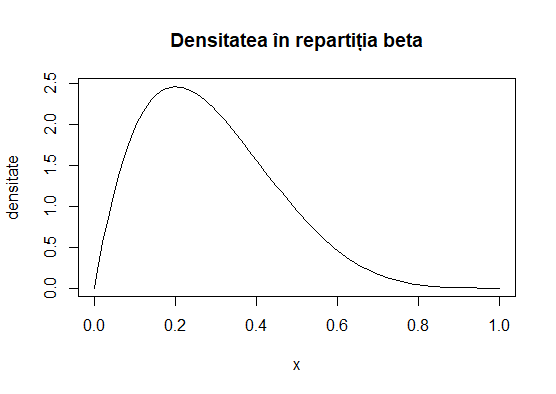
\includegraphics[scale=0.75]{DenBeta}
		\caption{den.beta(2, 5)}
	\end{figure}

	\begin{figure}[h!]
		\centering		
		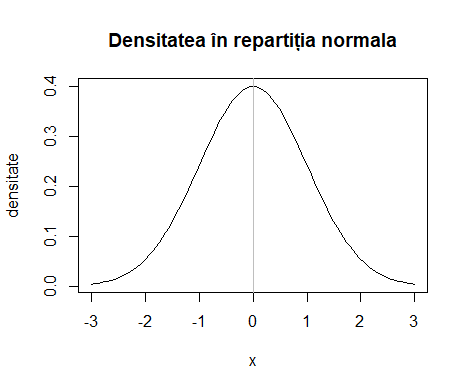
\includegraphics[scale=0.75]{DenNorm}
		\caption{den.normala(0, 1)}
	\end{figure}

	\begin{figure}
		\centering
		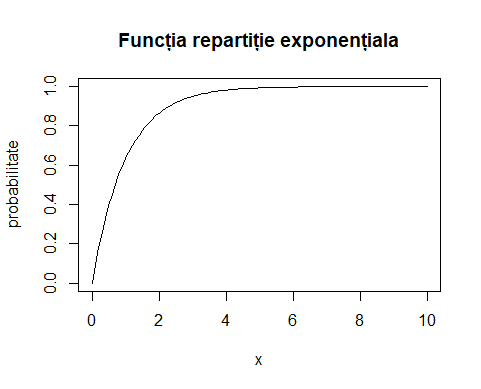
\includegraphics[scale=0.75]{RepExp}
		\caption{rep.exponentiala(1)}	
	\end{figure}

	\begin{figure}
		\centering
		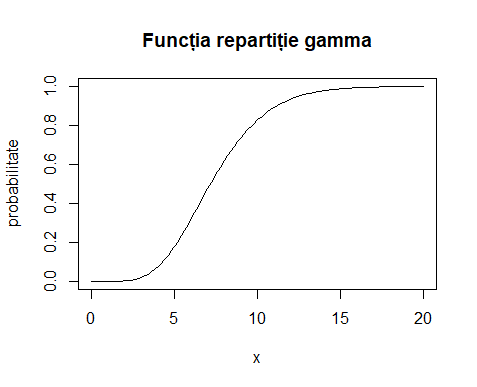
\includegraphics[scale=0.75]{RepGamma}
		\caption{rep.gamma(7.5, 1)}	
	\end{figure}
	
\end{document}